\documentclass[a4paper,12pt]{article}

\title{Biology 30 IB \\ Nervous System}
\author{Jad Chehimi}

% document setup
\renewcommand{\familydefault}{\sfdefault}
\linespread{1.25}
\usepackage[margin=1in]{geometry}
\usepackage{setspace}
\usepackage{enumitem}
\setlist{nosep}
\usepackage{color,soul}
\setcounter{secnumdepth}{0}

% tools
\usepackage[hidelinks]{hyperref}
\usepackage{float}
%% images
\usepackage{graphicx}
\graphicspath{ {./images/} }
%% science
\usepackage{siunitx}
%% chemistry
%\usepackage[version=4]{mhchem}

\begin{document}
\maketitle

% temp
\begin{center}
\Huge
Unfinished!
\normalsize
\end{center}
% temp

\tableofcontents

\pagebreak

\section{(13.1) The Nervous System}
\begin{itemize}
    \item{\textbf{Equilibrium/Homeostasis} = balance, main job of nervous system is to maintain this}
    \item{
            Nervous system contains...
            \begin{itemize}
                \item{Brain}
                \item{Spinal cord}
                \item{Nerves}
            \end{itemize}
        }
\end{itemize}

\section{Divisions of the Nervous System}
\begin{figure}[H]
    \centering
    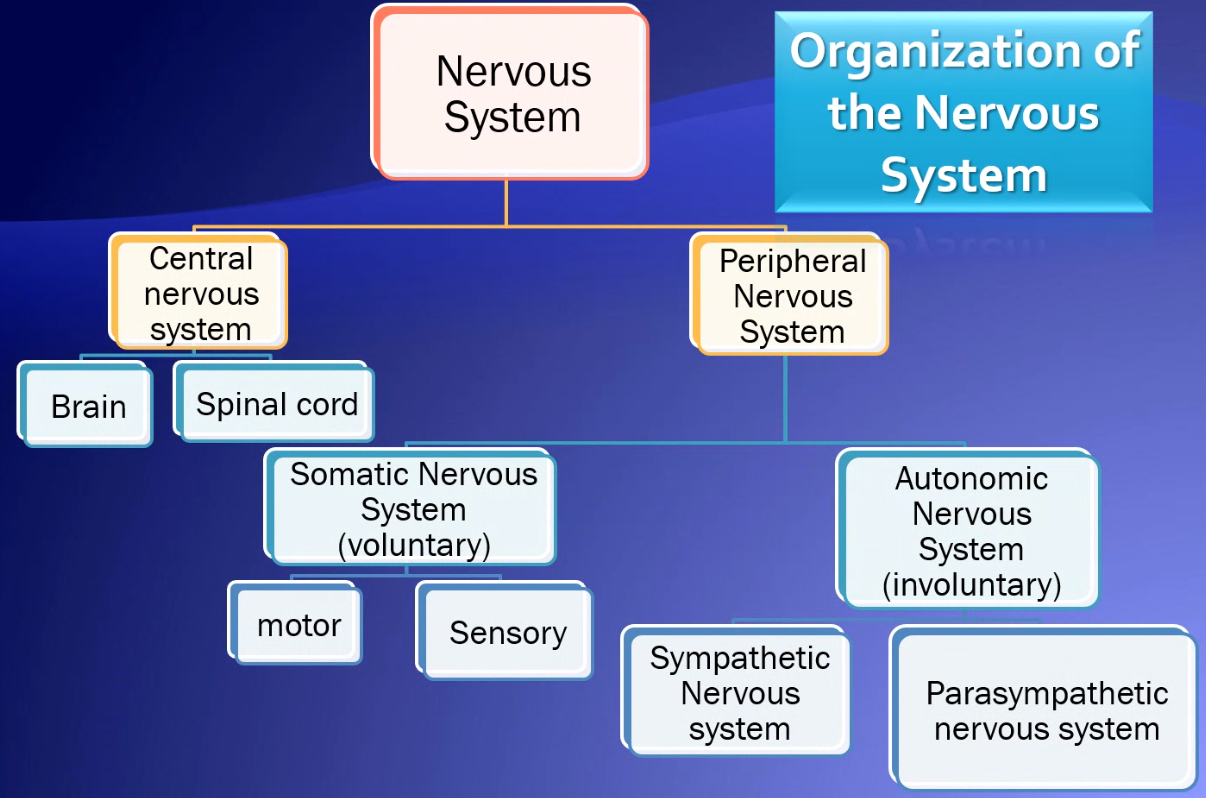
\includegraphics[width=\textwidth]{flowchart}
\end{figure}

\subsection{Central Nervous System (CNS)}
\begin{itemize}
    \item{Integrates and processes information}
    \item{Consists of \hl{brain} and \hl{spinal cord}}
\end{itemize}

\subsection{Peripheral Nervous System (PNS)}
\begin{itemize}
    \item{\hl{Messenger nerves}; bring \hl{info to and from} the central nervous system}
    \item{
            Each include two types of neurons...
            \begin{itemize}
                \item{\textbf{Sensory receptors} = carry sensory info to the CNS}
                \item{\textbf{Motor neurons} = \hl{voluntary motor/muscle control}, carry signals from the CNS to the skeletal muscles}
            \end{itemize}
        }

\end{itemize}

\subsubsection{Somatic Nervous System (SNS)}
\begin{itemize}
    \item{Voluntary control}
    \item{\hl{Somatic sensory neurons} gather info from external stimuli --- \hl{five senses}}
    \item{\hl{Somatic motor neurons} control voluntary skeletal muscles}
\end{itemize}

\subsubsection{Autonomic Nervous System (ANS)}
\begin{itemize}
    \item{Divisions of automatic nerves that are \hl{antagonistic/oppose each other}}
    \item{Regulates involuntary control processes (automatic), such as breathing and heartbeat}
    \item{\hl{Autonomic sensory neurons} gather info from internal stimuli --- involved with blood pressure and heart rate}
    \item{Autonomic motor neurons control glandular secretions and the function of \hl{smooth and cardiac muscles}}
                    \\
\end{itemize}

\textbf{Sympathetic Nervous System}
\begin{itemize}
    \item{"Fight or flight (or freeze)" responses}
    \item{\hl{Prioritizes urgent} functions, such as by speeding up rates of breathing, heart rate, etc.}
    \item{\hl{Disables non-urgent} functions, such as digesting}
        \\
\end{itemize}

\textbf{Parasympathetic Nervous System}
\begin{itemize}
    \item{"Rest and digest" responses}
    \item{\hl{Restores normal priorities} restored, slows down rates of breathing, heart rate, etc.}
    \item{\hl{Re-enables non-urgent} functions, such as digesting}
\end{itemize}

\pagebreak

\section{Cells of the Nervous System}
\subsection{Neurons}
Functional units of nervous system, \hl{tissues of neurons} are called \textbf{nerves}.
\begin{itemize}
    \item{\hl{Respond} to physical and chemical stimuli}
    \item{\hl{Conduct} electrochemical signals}
    \item{\hl{Release} chemicals that regulate various body processes}
\end{itemize}

\subsubsection{Types of Neurons}
\begin{itemize}
    \item{\textbf{Sensory receptors} = recieves info from 5 senses; bulb-like, end part of sensory neuron}
    \item{\textbf{Sensory neurons} = gather \hl{info from sensory} receptors, transmits \hl{to CNS}}
    \item{\textbf{Interneurons} = only in CNS; link \hl{between sensory and motor} neurons}
    \item{\textbf{Motor neurons} = transmt info from \hl{CNS to effectors}}
    \item{\textbf{Effectors} = muscles, glands, other organs}
\end{itemize}

\subsection{Glial Cells}
Supporting cells of nerve cells.
\begin{itemize}
    \item{Nourish neurons, remove wastes, \& defend against infection}
    \item{Provide a supporting framework for all nervous-system tissue}
\end{itemize}

\section{Neuron Anatomy}
\subsection{Dendrites}
\begin{itemize}
    \item{Short, branching terminals of neuron}
    \item{
            Recieve information from...
            \begin{itemize}
                \item{other neurons}
                \item{senses (making it a \textbf{sensory receptor})}
            \end{itemize}
        }
\end{itemize}

\subsection{Cell Body}
\begin{itemize}
    \item{Site of metabolic reactions}
    \item{Contains a nucleus to process info from dendrites}
    \item{Makes a decision}
\end{itemize}

\subsection{Axon}
\begin{itemize}
    \item{Thread-like component of neuron after cell body}
    \item{Conducts impulses away from the cell body}
    \item{Axon terminals = axon ends branch into many fibres}
\end{itemize}

\subsection{Myelin Sheath}
\begin{figure}[H]
    \centering
    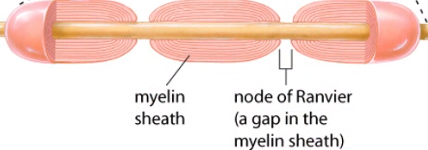
\includegraphics[width=0.50\textwidth]{ranvier}
\end{figure}

\begin{itemize}
    \item{Insulation on neurons; \hl{not all neurons} have myelin sheath}
    \item{\hl{Prevents loss} of charged \hl{ions}}
\end{itemize}

\subsubsection{Schwann Cells}
\begin{itemize}
    \item{Glial cells \hl{wrapping around axon}; wrapped form = myelin sheath}
    \item{\textbf{White matter} = \hl{myelinated/insulated} neurons; slower than grey}
    \item{\textbf{Grey matter} = \hl{unmyelinated/exposed} neurons; common on brain surface}
\end{itemize}

\subsubsection{Node of Ranvier}
\begin{itemize}
    \item{\hl{Gap} between myelin sheaths}
    \item{Nerve impulses \hl{"jump" from node to node}, speeding up movement}
    \item{
            \textbf{Neurilemma}
            \begin{itemize}
                \item{promotes the \hl{regeneration of damaged axons}}
                \item{some, \hl{not all}, schwann cells form this additional layer over the myelin sheath}
                \item{not present in unmyelianted, grey matter of CNS}
            \end{itemize}
        }
\end{itemize}

\section{Repairing Damage Nerves}
\subsection{Stem Cells}
\begin{itemize}
    \item{Unspecialized cells}
    \item{Can be used to repair all sorts of injuries}
\end{itemize}

\subsection{Reflex Arc}
\begin{itemize}
    \item{\hl{Prevents injury} before even being consciously aware of a threat}
    \item{\textbf{Reflexes} = sudden, unlearned, and involuntary responses to certain stimuli}
    \item{
            \textbf{Spinal Reflex}
            \begin{itemize}
                \item{Reflex with no brain involvement during threat}
                \item{Decision to reflex made by interneuron}
                \item{Interneuron communicates to brain after threat}
                \item{Occurs for spinal reflexes AND conditional reflexes (e.g. touching something hot)}
                \item{Stimulus \\ $\longrightarrow$ Sensory Receptor (dendrite) $\longrightarrow$ Sensory Neuron $\longrightarrow$ Interneuron (in spine) $\longrightarrow$ Motor Neuron $\longrightarrow$ Effector Organ $\longrightarrow$ Response}
            \end{itemize}
        }
\end{itemize}

\end{document}
